% Options for packages loaded elsewhere
\PassOptionsToPackage{unicode}{hyperref}
\PassOptionsToPackage{hyphens}{url}
\PassOptionsToPackage{dvipsnames,svgnames,x11names}{xcolor}
%
\documentclass[
  letterpaper,
  DIV=11,
  numbers=noendperiod]{scrartcl}

\usepackage{amsmath,amssymb}
\usepackage{iftex}
\ifPDFTeX
  \usepackage[T1]{fontenc}
  \usepackage[utf8]{inputenc}
  \usepackage{textcomp} % provide euro and other symbols
\else % if luatex or xetex
  \usepackage{unicode-math}
  \defaultfontfeatures{Scale=MatchLowercase}
  \defaultfontfeatures[\rmfamily]{Ligatures=TeX,Scale=1}
\fi
\usepackage{lmodern}
\ifPDFTeX\else  
    % xetex/luatex font selection
\fi
% Use upquote if available, for straight quotes in verbatim environments
\IfFileExists{upquote.sty}{\usepackage{upquote}}{}
\IfFileExists{microtype.sty}{% use microtype if available
  \usepackage[]{microtype}
  \UseMicrotypeSet[protrusion]{basicmath} % disable protrusion for tt fonts
}{}
\makeatletter
\@ifundefined{KOMAClassName}{% if non-KOMA class
  \IfFileExists{parskip.sty}{%
    \usepackage{parskip}
  }{% else
    \setlength{\parindent}{0pt}
    \setlength{\parskip}{6pt plus 2pt minus 1pt}}
}{% if KOMA class
  \KOMAoptions{parskip=half}}
\makeatother
\usepackage{xcolor}
\setlength{\emergencystretch}{3em} % prevent overfull lines
\setcounter{secnumdepth}{-\maxdimen} % remove section numbering
% Make \paragraph and \subparagraph free-standing
\makeatletter
\ifx\paragraph\undefined\else
  \let\oldparagraph\paragraph
  \renewcommand{\paragraph}{
    \@ifstar
      \xxxParagraphStar
      \xxxParagraphNoStar
  }
  \newcommand{\xxxParagraphStar}[1]{\oldparagraph*{#1}\mbox{}}
  \newcommand{\xxxParagraphNoStar}[1]{\oldparagraph{#1}\mbox{}}
\fi
\ifx\subparagraph\undefined\else
  \let\oldsubparagraph\subparagraph
  \renewcommand{\subparagraph}{
    \@ifstar
      \xxxSubParagraphStar
      \xxxSubParagraphNoStar
  }
  \newcommand{\xxxSubParagraphStar}[1]{\oldsubparagraph*{#1}\mbox{}}
  \newcommand{\xxxSubParagraphNoStar}[1]{\oldsubparagraph{#1}\mbox{}}
\fi
\makeatother

\usepackage{color}
\usepackage{fancyvrb}
\newcommand{\VerbBar}{|}
\newcommand{\VERB}{\Verb[commandchars=\\\{\}]}
\DefineVerbatimEnvironment{Highlighting}{Verbatim}{commandchars=\\\{\}}
% Add ',fontsize=\small' for more characters per line
\usepackage{framed}
\definecolor{shadecolor}{RGB}{241,243,245}
\newenvironment{Shaded}{\begin{snugshade}}{\end{snugshade}}
\newcommand{\AlertTok}[1]{\textcolor[rgb]{0.68,0.00,0.00}{#1}}
\newcommand{\AnnotationTok}[1]{\textcolor[rgb]{0.37,0.37,0.37}{#1}}
\newcommand{\AttributeTok}[1]{\textcolor[rgb]{0.40,0.45,0.13}{#1}}
\newcommand{\BaseNTok}[1]{\textcolor[rgb]{0.68,0.00,0.00}{#1}}
\newcommand{\BuiltInTok}[1]{\textcolor[rgb]{0.00,0.23,0.31}{#1}}
\newcommand{\CharTok}[1]{\textcolor[rgb]{0.13,0.47,0.30}{#1}}
\newcommand{\CommentTok}[1]{\textcolor[rgb]{0.37,0.37,0.37}{#1}}
\newcommand{\CommentVarTok}[1]{\textcolor[rgb]{0.37,0.37,0.37}{\textit{#1}}}
\newcommand{\ConstantTok}[1]{\textcolor[rgb]{0.56,0.35,0.01}{#1}}
\newcommand{\ControlFlowTok}[1]{\textcolor[rgb]{0.00,0.23,0.31}{\textbf{#1}}}
\newcommand{\DataTypeTok}[1]{\textcolor[rgb]{0.68,0.00,0.00}{#1}}
\newcommand{\DecValTok}[1]{\textcolor[rgb]{0.68,0.00,0.00}{#1}}
\newcommand{\DocumentationTok}[1]{\textcolor[rgb]{0.37,0.37,0.37}{\textit{#1}}}
\newcommand{\ErrorTok}[1]{\textcolor[rgb]{0.68,0.00,0.00}{#1}}
\newcommand{\ExtensionTok}[1]{\textcolor[rgb]{0.00,0.23,0.31}{#1}}
\newcommand{\FloatTok}[1]{\textcolor[rgb]{0.68,0.00,0.00}{#1}}
\newcommand{\FunctionTok}[1]{\textcolor[rgb]{0.28,0.35,0.67}{#1}}
\newcommand{\ImportTok}[1]{\textcolor[rgb]{0.00,0.46,0.62}{#1}}
\newcommand{\InformationTok}[1]{\textcolor[rgb]{0.37,0.37,0.37}{#1}}
\newcommand{\KeywordTok}[1]{\textcolor[rgb]{0.00,0.23,0.31}{\textbf{#1}}}
\newcommand{\NormalTok}[1]{\textcolor[rgb]{0.00,0.23,0.31}{#1}}
\newcommand{\OperatorTok}[1]{\textcolor[rgb]{0.37,0.37,0.37}{#1}}
\newcommand{\OtherTok}[1]{\textcolor[rgb]{0.00,0.23,0.31}{#1}}
\newcommand{\PreprocessorTok}[1]{\textcolor[rgb]{0.68,0.00,0.00}{#1}}
\newcommand{\RegionMarkerTok}[1]{\textcolor[rgb]{0.00,0.23,0.31}{#1}}
\newcommand{\SpecialCharTok}[1]{\textcolor[rgb]{0.37,0.37,0.37}{#1}}
\newcommand{\SpecialStringTok}[1]{\textcolor[rgb]{0.13,0.47,0.30}{#1}}
\newcommand{\StringTok}[1]{\textcolor[rgb]{0.13,0.47,0.30}{#1}}
\newcommand{\VariableTok}[1]{\textcolor[rgb]{0.07,0.07,0.07}{#1}}
\newcommand{\VerbatimStringTok}[1]{\textcolor[rgb]{0.13,0.47,0.30}{#1}}
\newcommand{\WarningTok}[1]{\textcolor[rgb]{0.37,0.37,0.37}{\textit{#1}}}

\providecommand{\tightlist}{%
  \setlength{\itemsep}{0pt}\setlength{\parskip}{0pt}}\usepackage{longtable,booktabs,array}
\usepackage{calc} % for calculating minipage widths
% Correct order of tables after \paragraph or \subparagraph
\usepackage{etoolbox}
\makeatletter
\patchcmd\longtable{\par}{\if@noskipsec\mbox{}\fi\par}{}{}
\makeatother
% Allow footnotes in longtable head/foot
\IfFileExists{footnotehyper.sty}{\usepackage{footnotehyper}}{\usepackage{footnote}}
\makesavenoteenv{longtable}
\usepackage{graphicx}
\makeatletter
\def\maxwidth{\ifdim\Gin@nat@width>\linewidth\linewidth\else\Gin@nat@width\fi}
\def\maxheight{\ifdim\Gin@nat@height>\textheight\textheight\else\Gin@nat@height\fi}
\makeatother
% Scale images if necessary, so that they will not overflow the page
% margins by default, and it is still possible to overwrite the defaults
% using explicit options in \includegraphics[width, height, ...]{}
\setkeys{Gin}{width=\maxwidth,height=\maxheight,keepaspectratio}
% Set default figure placement to htbp
\makeatletter
\def\fps@figure{htbp}
\makeatother

\KOMAoption{captions}{tableheading}
\makeatletter
\@ifpackageloaded{tcolorbox}{}{\usepackage[skins,breakable]{tcolorbox}}
\@ifpackageloaded{fontawesome5}{}{\usepackage{fontawesome5}}
\definecolor{quarto-callout-color}{HTML}{909090}
\definecolor{quarto-callout-note-color}{HTML}{0758E5}
\definecolor{quarto-callout-important-color}{HTML}{CC1914}
\definecolor{quarto-callout-warning-color}{HTML}{EB9113}
\definecolor{quarto-callout-tip-color}{HTML}{00A047}
\definecolor{quarto-callout-caution-color}{HTML}{FC5300}
\definecolor{quarto-callout-color-frame}{HTML}{acacac}
\definecolor{quarto-callout-note-color-frame}{HTML}{4582ec}
\definecolor{quarto-callout-important-color-frame}{HTML}{d9534f}
\definecolor{quarto-callout-warning-color-frame}{HTML}{f0ad4e}
\definecolor{quarto-callout-tip-color-frame}{HTML}{02b875}
\definecolor{quarto-callout-caution-color-frame}{HTML}{fd7e14}
\makeatother
\makeatletter
\@ifpackageloaded{caption}{}{\usepackage{caption}}
\AtBeginDocument{%
\ifdefined\contentsname
  \renewcommand*\contentsname{Table of contents}
\else
  \newcommand\contentsname{Table of contents}
\fi
\ifdefined\listfigurename
  \renewcommand*\listfigurename{List of Figures}
\else
  \newcommand\listfigurename{List of Figures}
\fi
\ifdefined\listtablename
  \renewcommand*\listtablename{List of Tables}
\else
  \newcommand\listtablename{List of Tables}
\fi
\ifdefined\figurename
  \renewcommand*\figurename{Figure}
\else
  \newcommand\figurename{Figure}
\fi
\ifdefined\tablename
  \renewcommand*\tablename{Table}
\else
  \newcommand\tablename{Table}
\fi
}
\@ifpackageloaded{float}{}{\usepackage{float}}
\floatstyle{ruled}
\@ifundefined{c@chapter}{\newfloat{codelisting}{h}{lop}}{\newfloat{codelisting}{h}{lop}[chapter]}
\floatname{codelisting}{Listing}
\newcommand*\listoflistings{\listof{codelisting}{List of Listings}}
\makeatother
\makeatletter
\makeatother
\makeatletter
\@ifpackageloaded{caption}{}{\usepackage{caption}}
\@ifpackageloaded{subcaption}{}{\usepackage{subcaption}}
\makeatother

\ifLuaTeX
  \usepackage{selnolig}  % disable illegal ligatures
\fi
\usepackage{bookmark}

\IfFileExists{xurl.sty}{\usepackage{xurl}}{} % add URL line breaks if available
\urlstyle{same} % disable monospaced font for URLs
\hypersetup{
  pdftitle={Introduction to Bayesian inference},
  pdfauthor={---},
  colorlinks=true,
  linkcolor={blue},
  filecolor={Maroon},
  citecolor={Blue},
  urlcolor={Blue},
  pdfcreator={LaTeX via pandoc}}


\title{Introduction to Bayesian inference}
\usepackage{etoolbox}
\makeatletter
\providecommand{\subtitle}[1]{% add subtitle to \maketitle
  \apptocmd{\@title}{\par {\large #1 \par}}{}{}
}
\makeatother
\subtitle{End of course data analysis project}
\author{---}
\date{}

\begin{document}
\maketitle


\section{Vaccination against
Varicella}\label{vaccination-against-varicella}

The Center for Disease Control (CDC) reports the vaccination coverage of
Varicella among young children. Varicella, commonly known as chicken-
pox, is a highly contagious viral infection caused by the
varicella-zoster virus (VZV). Vaccination against chickenpox has been
highly effective in reducing the incidence and severity of the disease.
In the United States, vaccination against varicella has been part of the
routine childhood immunization sched- ule since the mid-1990s. Since the
vaccine's introduction, there has been a dramatic decline in the number
of chickenpox cases, hospitalizations, and deaths associated with the
disease. The target for vaccination coverage of varicella (chickenpox)
in the United States, as set by the Centers for Dis- ease Control and
Prevention (CDC), is typically around 90\% or higher for children. This
high coverage rate is aimed at achieving herd immunity and preventing
outbreaks of chickenpox within communities.

\section{Project 1: Insurance}\label{project-1-insurance}

The next table summarizes, based on a survey, the number of children in
the birth cohort 2014-2017 that had at least one dose of the Varicella
vaccine. It gives the number of vaccinated children (Vaccinated) amongst
the number of children in the survey (Sample Size). The information is
provided for 5 regions of the US, and split according to insurance
status (private insurance, uninsured or any Medicaid

\begin{longtable}[]{@{}llll@{}}
\toprule\noalign{}
Geography & Insurance & Vaccinated & Sample Size \\
\midrule\noalign{}
\endhead
\bottomrule\noalign{}
\endlastfoot
North Carolina & Any Medicaid & 380 & 419 \\
North Carolina & Private Insurance Only & 632 & 673 \\
North Carolina & Uninsured & 28 & 34 \\
Georgia & Any Medicaid & 363 & 396 \\
Georgia & Private Insurance Only & 527 & 576 \\
Georgia & Uninsured & 36 & 50 \\
Wisconsin & Any Medicaid & 282 & 332 \\
Wisconsin & Private Insurance Only & 514 & 548 \\
Wisconsin & Uninsured & 16 & 34 \\
Florida & Any Medicaid & 446 & 490 \\
Florida & Private Insurance Only & 588 & 628 \\
Florida & Uninsured & 28 & 39 \\
Mississippi & Private Insurance Only & 400 & 441 \\
Mississippi & Uninsured & 27 & 32 \\
\end{longtable}

\section{Question 1}\label{question-1}

\begin{tcolorbox}[enhanced jigsaw, bottomrule=.15mm, colback=white, opacityback=0, left=2mm, colframe=quarto-callout-color-frame, toprule=.15mm, leftrule=.75mm, rightrule=.15mm, arc=.35mm, breakable]

Derive analytically the posterior of the vaccination coverage per ge-
ography and insurance group. Use a conjugate prior that (1) reflects no
knowledge on the vaccination coverage, and (2) reflects that vac-
cination coverage is typically around 90\% or higher. Give posterior
summary measures of the vaccination coverage per geography and in-
surance group. Is the choice of the prior impacting your results?

\end{tcolorbox}

\subsection{Theoretical
considerations}\label{theoretical-considerations}

The outcome \emph{Vaccinated/Not Vaccinated} follows a Bernouilli
distribution with parameter \(p\):

\(V:\) Vaccination status \(V \in \{0,1\}\) \(V \sim \mathcal{Bern}(p)\)

It is known from theory that the sum of \(n\) \(i.i.d\) Bernoulli random
variables follows a Binomial distribution. This will be used to model
the sample outcome: the number of vaccinated people \(V_s\) in a random
sample of size \(n\):

\[V_s = \sum_i^n V_i \sim \mathcal{Binom}(n, \theta)\]

where \(\theta\) is the parameter of interest - the vaccine coverage.

In the course, we saw that the Beta distribution is the conjugate prior
for binomially distributed data:

\begin{longtable}[]{@{}
  >{\raggedright\arraybackslash}p{(\columnwidth - 2\tabcolsep) * \real{0.6000}}
  >{\raggedright\arraybackslash}p{(\columnwidth - 2\tabcolsep) * \real{0.4000}}@{}}
\toprule\noalign{}
\begin{minipage}[b]{\linewidth}\raggedright
Distribution
\end{minipage} & \begin{minipage}[b]{\linewidth}\raggedright
Formula
\end{minipage} \\
\midrule\noalign{}
\endhead
\bottomrule\noalign{}
\endlastfoot
Prior & \(p(\theta) = \mathcal{Beta}(\alpha, \beta)\) \\
Likelihood &
\(p(y \mid \theta) = {n \choose k} \theta^k (1 - \theta)^{n-k}\) \\
Posterior &
\(p(\theta \mid y) = \mathcal{Beta}(\alpha + k, \beta + n - k)\) \\
\end{longtable}

The summary measures for the Beta distribution are defined as follows:

\begin{longtable}[]{@{}
  >{\raggedright\arraybackslash}p{(\columnwidth - 2\tabcolsep) * \real{0.6667}}
  >{\raggedright\arraybackslash}p{(\columnwidth - 2\tabcolsep) * \real{0.3333}}@{}}
\toprule\noalign{}
\begin{minipage}[b]{\linewidth}\raggedright
Summary Measure
\end{minipage} & \begin{minipage}[b]{\linewidth}\raggedright
Formula
\end{minipage} \\
\midrule\noalign{}
\endhead
\bottomrule\noalign{}
\endlastfoot
Mean & \(\frac{\alpha}{\alpha + \beta}\) \\
Median & See Note \\
Mode & \(\frac{\alpha - 1}{\alpha + \beta - 2}\) for
\(\alpha, \beta > 1\) \\
\end{longtable}

Note: The median of the Beta distribution does not have a simple closed
form expression. It can be approximated numerically or using statistical
software.

\begin{Shaded}
\begin{Highlighting}[]
\FunctionTok{source}\NormalTok{(}\StringTok{"./project.R"}\NormalTok{)}
\end{Highlighting}
\end{Shaded}

\begin{verbatim}

Attaching package: 'dplyr'
\end{verbatim}

\begin{verbatim}
The following objects are masked from 'package:stats':

    filter, lag
\end{verbatim}

\begin{verbatim}
The following objects are masked from 'package:base':

    intersect, setdiff, setequal, union
\end{verbatim}

\subsection{Choice of prior
distributions}\label{choice-of-prior-distributions}

\subsubsection{(1) No prior knowledge}\label{no-prior-knowledge}

In order to reflect no prior knowledge on the vaccine coverage, the
weakly-informative prior Beta(1,1) will be used, which is equivalent to
the uniform distribution over \(\[1,1\]\).

\subsubsection{(2) Vaccine coverage
\textgreater90\%}\label{vaccine-coverage-90}

For modeling prior knowledge that vaccine coverage is about 90\%, we
chose the Beta(150, 7) distribution.

\subsubsection{Comparison of priors}\label{comparison-of-priors}

\begin{Shaded}
\begin{Highlighting}[]
\NormalTok{plot\_priors}
\end{Highlighting}
\end{Shaded}

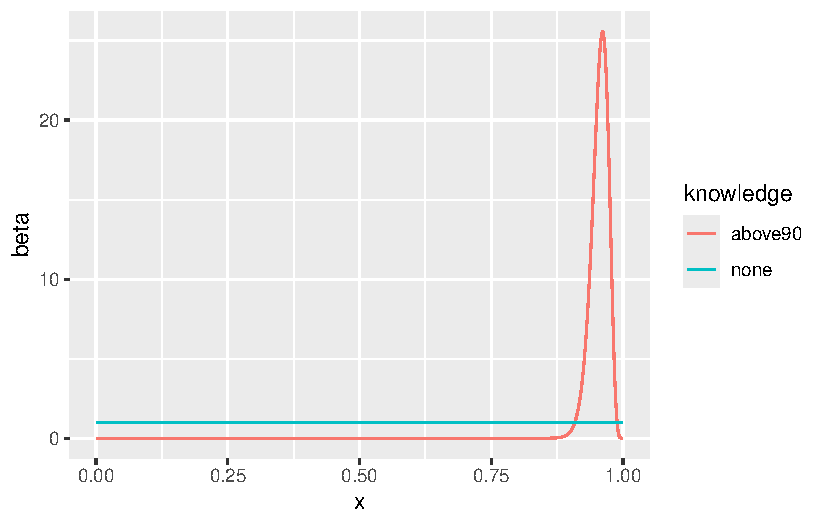
\includegraphics{project_files/figure-pdf/unnamed-chunk-2-1.pdf}

\subsection{Results}\label{results}

\begin{Shaded}
\begin{Highlighting}[]
\NormalTok{uni\_posterior }\SpecialCharTok{\%\textgreater{}\%}\NormalTok{ knitr}\SpecialCharTok{::}\FunctionTok{kable}\NormalTok{(}\AttributeTok{caption =} \StringTok{"Posterior distribution parameters and summary measures per geography and insurance for Beta(1,1) prior"}\NormalTok{)}
\end{Highlighting}
\end{Shaded}

\begin{longtable}[]{@{}
  >{\raggedright\arraybackslash}p{(\columnwidth - 10\tabcolsep) * \real{0.2083}}
  >{\raggedright\arraybackslash}p{(\columnwidth - 10\tabcolsep) * \real{0.3194}}
  >{\raggedleft\arraybackslash}p{(\columnwidth - 10\tabcolsep) * \real{0.0972}}
  >{\raggedleft\arraybackslash}p{(\columnwidth - 10\tabcolsep) * \real{0.0972}}
  >{\raggedleft\arraybackslash}p{(\columnwidth - 10\tabcolsep) * \real{0.1389}}
  >{\raggedleft\arraybackslash}p{(\columnwidth - 10\tabcolsep) * \real{0.1389}}@{}}
\caption{Posterior distribution parameters and summary measures per
geography and insurance for Beta(1,1) prior}\tabularnewline
\toprule\noalign{}
\begin{minipage}[b]{\linewidth}\raggedright
Geography
\end{minipage} & \begin{minipage}[b]{\linewidth}\raggedright
Insurance
\end{minipage} & \begin{minipage}[b]{\linewidth}\raggedleft
post\_a
\end{minipage} & \begin{minipage}[b]{\linewidth}\raggedleft
post\_b
\end{minipage} & \begin{minipage}[b]{\linewidth}\raggedleft
post\_mean
\end{minipage} & \begin{minipage}[b]{\linewidth}\raggedleft
post\_mode
\end{minipage} \\
\midrule\noalign{}
\endfirsthead
\toprule\noalign{}
\begin{minipage}[b]{\linewidth}\raggedright
Geography
\end{minipage} & \begin{minipage}[b]{\linewidth}\raggedright
Insurance
\end{minipage} & \begin{minipage}[b]{\linewidth}\raggedleft
post\_a
\end{minipage} & \begin{minipage}[b]{\linewidth}\raggedleft
post\_b
\end{minipage} & \begin{minipage}[b]{\linewidth}\raggedleft
post\_mean
\end{minipage} & \begin{minipage}[b]{\linewidth}\raggedleft
post\_mode
\end{minipage} \\
\midrule\noalign{}
\endhead
\bottomrule\noalign{}
\endlastfoot
North Carolina & Any Medicaid & 381 & 40 & 0.9049881 & 0.9069212 \\
North Carolina & Private Insurance Only & 633 & 42 & 0.9377778 &
0.9390788 \\
North Carolina & Uninsured & 29 & 7 & 0.8055556 & 0.8235294 \\
Georgia & Any Medicaid & 364 & 34 & 0.9145729 & 0.9166667 \\
Georgia & Private Insurance Only & 528 & 50 & 0.9134948 & 0.9149306 \\
Georgia & Uninsured & 37 & 15 & 0.7115385 & 0.7200000 \\
Wisconsin & Any Medicaid & 283 & 51 & 0.8473054 & 0.8493976 \\
Wisconsin & Private Insurance Only & 515 & 35 & 0.9363636 & 0.9379562 \\
Wisconsin & Uninsured & 17 & 19 & 0.4722222 & 0.4705882 \\
Florida & Any Medicaid & 447 & 45 & 0.9085366 & 0.9102041 \\
Florida & Private Insurance Only & 589 & 41 & 0.9349206 & 0.9363057 \\
Florida & Uninsured & 29 & 12 & 0.7073171 & 0.7179487 \\
Mississippi & Private Insurance Only & 401 & 42 & 0.9051919 &
0.9070295 \\
Mississippi & Uninsured & 28 & 6 & 0.8235294 & 0.8437500 \\
\end{longtable}




\end{document}
